\documentclass[USenglish]{scrbook}

\usepackage{graphicx}
\graphicspath{
                          {figures/}
                          {../NSD/}
                         }
\DeclareGraphicsExtensions{.pdf,.png}
\usepackage[authoryear,sort&compress]{natbib}
\usepackage[usenames,dvipsnames]{color}
\usepackage[pdftex,                                     % hyper-references for pdftex
bookmarksnumbered=true,%                       % generate bookmarks with numbers
pagebackref=true,%                                      % generate backref in biblio
colorlinks=true,%
linkcolor=MidnightBlue,%
citecolor=MidnightBlue,%
breaklinks=true,%
]{hyperref}%

 \hypersetup{
pdfauthor   = {Claudio Zambaldi, Philip Eisenlohr},
pdftitle    = {Manual to the Crystal Plasticity Finite Element Subroutine developed at the Max-Planck-Institut f\"ur Eisenforschung},
pdfsubject  = {},
pdfkeywords = {},
pdfcreator  = {},
pdfproducer = {pdftex}%,
%pdfpagemode={FullScreen}
}


\usepackage{amsmath,amssymb,amsfonts}
\usepackage{bm}
\usepackage{miller}
\usepackage[alsoload={accepted,named,prefix}]{siunitx}
\usepackage{booktabs}
\usepackage{longtable}
\usepackage[indent,bf,tableposition=top]{caption}    % Einstellen des caption-Stils, war caption2
\usepackage[format=hang]{subfig}
\usepackage{tocbibind}
\usepackage[bookman]{quotchap}
\usepackage{csquotes} % consistent quoting by \enquote{...}
\usepackage{listings}
\lstloadlanguages{fortran}
\lstset{language={},
  frame=none,
  xleftmargin=10mm,
  xrightmargin=10mm,
	numbers=left,
	stepnumber=1,
	numbersep=5pt,
	numberstyle=\tiny,
	breaklines=true,
	breakautoindent=true,
	postbreak=...,%\space,
	tabsize=2,
	basicstyle=\ttfamily\footnotesize,
	showspaces=false,
	showstringspaces=false,
	extendedchars=true,
	backgroundcolor=\color{white}
}


\newlength{\diagramsize}
\setlength{\diagramsize}{0.9\textwidth}

\setcounter{tocdepth}{2}

\newcommand{\includepath}{include}

\newcommand{\ie}{\textit{i.e.}}
\newcommand{\eg}{\textit{e.g.}}
\newcommand{\cf}{\textit{cf.}}
\newcommand{\etal}{\textit{et al.}}
\newcommand{\Euler}{\textsc{Euler}}
\newcommand{\OneD}{\hbox{1-D}}
\newcommand{\TwoD}{\hbox{2-D}}
\newcommand{\ThreeD}{\hbox{3-D}}

\DeclareMathOperator{\sign}{sgn}
\DeclareMathOperator{\divergence}{div}
\DeclareMathOperator{\grad}{grad}
\DeclareMathOperator{\curl}{curl}
\DeclareMathOperator{\Divergence}{Div}
\DeclareMathOperator{\Grad}{Grad}
\DeclareMathOperator{\Curl}{Curl}

\newcommand{\tnsr}[1]{\ensuremath{\bm{#1}}}
\newcommand{\vctr}[1]{\ensuremath{\bm{#1}}}

\newcommand{\drv}{\ensuremath{\mathrm d}}

\newcommand{\transpose}[1]{\ensuremath{{#1}^{\mathrm T}}}
\newcommand{\inverse}[1]{\ensuremath{{#1}^{-1}}}
\newcommand{\invtranspose}[1]{\ensuremath{{#1}^{\mathrm{-T}}}}

\newcommand{\eyetwo}{\ensuremath{\tnsr{I}}}
\newcommand{\eyefour}{\ensuremath{\mathbb{I}}}
\newcommand{\F}{\ensuremath{\tnsr F}}
\newcommand{\Fp}{\ensuremath{\tnsr F_\text{p}}}
\newcommand{\Fe}{\ensuremath{\tnsr F _\text{e}}}
\newcommand{\Ftr}{\ensuremath{\tnsr F _\text{tr}}}
\newcommand{\E}{\ensuremath{\tnsr E}}
\newcommand{\GL}{\ensuremath{\tnsr E_\text{e}}}
\newcommand{\fPK}{\ensuremath{\tnsr P}}
\newcommand{\sPK}{\ensuremath{\tnsr S}}
\newcommand{\etap}{\ensuremath{\eta_\text{p}}}
\newcommand{\etae}{\ensuremath{\eta_\text{e}}}
\newcommand{\etatr}{\ensuremath{\eta_\text{tr}}}
\newcommand{\dtF}{\ensuremath{\dot{\tnsr F}}}
\newcommand{\dtFp}{\ensuremath{\dot{\tnsr F}_\text{p}}}
\newcommand{\dtFe}{\ensuremath{\dot{\tnsr F}_\text{e}}}
\newcommand{\dtetap}{\ensuremath{\dot{\eta}_\text{p}}}
\newcommand{\Lp}{\ensuremath{\tnsr L_\text{p}}}
\newcommand{\Je}{\ensuremath{J_\text{e}}}
\newcommand{\Jtr}{\ensuremath{J_\text{tr}}}
\newcommand{\thetatr}{\ensuremath{\theta_\text{tr}}}
\newcommand{\Elasticity}{\ensuremath{\mathbb{C}}}
\newcommand{\Cauchy}{\ensuremath{\boldsymbol{\sigma}}}
\newcommand{\Ntwin}{\ensuremath{N_\text{twin}}}
\newcommand{\Nslip}{\ensuremath{N_\text{slip}}}
\newcommand{\testfnc}{\ensuremath{\delta\vctr v}}

% Reference formats
\newcommand{\fref}[1]{figure~\ref{#1}}             % figure x
\newcommand{\Fref}[1]{Figure~\ref{#1}}             % Figure x
\newcommand{\fsref}[1]{figures~\ref{#1}}           % figures x
\newcommand{\Fsref}[1]{Figures~\ref{#1}}           % Figures x

\newcommand{\tref}[1]{table~\ref{#1}}              % tabke x
\newcommand{\Tref}[1]{Table~\ref{#1}}              % Table x
\newcommand{\tsref}[1]{tables~\ref{#1}}            % tables x
\newcommand{\Tsref}[1]{Tables~\ref{#1}}            % Tables x

\newcommand{\eref}[1]{equation~\eqref{#1}}         % equation (x)
\newcommand{\Eref}[1]{Equation~\eqref{#1}}         % Equation (x)
\newcommand{\esref}[1]{equations~\eqref{#1}}       % equations (x)
\newcommand{\Esref}[1]{Equations~\eqref{#1}}       % Equations (x)

\newcommand{\cref}[1]{chapter~\ref{#1}}            % chapter x
\newcommand{\Cref}[1]{Chapter~\ref{#1}}            % Chapter x
\newcommand{\csref}[1]{chapters~\ref{#1}}          % chapters x
\newcommand{\Csref}[1]{Chapters~\ref{#1}}          % Chapters x

\newcommand{\sref}[1]{section~\ref{#1}}            % section x
\newcommand{\Sref}[1]{Section~\ref{#1}}            % Section x
\newcommand{\ssref}[1]{sections~\ref{#1}}          % sections x
\newcommand{\Ssref}[1]{Sections~\ref{#1}}          % Sections x

% text formatting
\newcommand{\term}[1]{\emph{#1}}
\newcommand{\reminder}[1]{\textcolor{Red}{#1}}
\newcommand{\remark}[1]{\textcolor{CornflowerBlue}{#1}}

% Change Layout of Backref
\renewcommand*{\backref}[1]{%
% default interface
% #1: backref list
%
% We want to use the alternative interface,
% therefore the definition is empty here.
}%
\renewcommand*{\backrefalt}[4]{%
% alternative interface
% #1: number of distinct back references
% #2: backref list with distinct entries
% #3: number of back references including duplicates
% #4: backref list including duplicates

\scriptsize
\begin{flushright}
Cited%
%~#3 %
%\ifnum#3=1 %
%time%
%\else
%times%
%\fi
~on %
\ifnum#1=1 %
page%
\else
pages%
\fi
~#2%
.%
\end{flushright}
}


\begin{document}
\title{Manual\\[1cm]\LARGE to the \\[3mm] Crystal Plasticity Finite Element Subroutine \\[3mm] developed at the \\[3mm] Max-Planck-Institut f\"ur Eisenforschung}
\author{Claudio Zambaldi \and Philip Eisenlohr}
\maketitle

%\includeonly{}

\frontmatter
%\include{foreword}
\tableofcontents
\listoftables
\listoffigures
%\include{include/preface}
\mainmatter

\renewcommand{\chaptermark}[1]{\markboth{{\thechapter\ \ #1}}{}}

% #################
\chapter{Preliminaries}
% #################

\section{Introduction}
For the theory and some application examples, see \citet{Roters2010}.

\section{History of the code}
?, spaghetti version, 

\section{Accessing the version controlled subroutine}
% This section is copied from the msuwiki: http://msusrv4/msuwiki/Theory%20and%20Simulation/SVN
Before you start: Before you are able to access the version-controlled software, you need to get a valid login to the msuhp9 server. Please ask either Berthold Becksch\"afer (-922) or Achim Kuhl (-923) to set up your permissions accordingly. 

\subsection{Windows}
\subsubsection{Putty}
Get yourself PuTTY and PuTTYgen from http://www.chiark.greenend.org.uk/~sgtatham/putty/download.html 
Generate a RSA (SSH2) 2048 bit strong key pair with PuTTYgen. Save the private part of the key to a secure location (My Documents or such). Copy the public part from the PuTTYgen window, paste it into a text-editor and save. Append the contents of that file to \verb|~/.ssh/authorized_keys| on any workstation you can log on to. 
Create a profile in PuTTY called "msuhp9" with host: msuhp9.mpie.de, your standard "MPIE\\myName" username and specify the above location of your private key file as means of authentication. 
You should then be able to connect with this profile to msuhp9 WITHOUT password authentication! 

\subsubsection{Tortoise}
Install the subversion-client Tortoise at http://tortoisesvn.net/downloads 
Create a directory to hold the CPFEM subroutine on your PC. 

Right-Click in this folder and select "SVN checkout" from the context menu. Specify 
svn+ssh://msuhp9/home/svn/repos/cpfem

as the URL of the desired repository. This will use the profile named "msuhp9" from PuTTY and should hence not ask for any authentication from your end.

\subsection{Linux workstations}

\subsubsection{Key authentication}
if not already done, generate a 2048 bit RSA key pair using 
ssh-keygen -t rsa -b 2048 
and go for the standard options offered. This will create "id\_rsa" (private key) and "id\_rsa.pub" (public key) within your \verb|~/.ssh| folder.

Append \verb|id_rsa.pub| to \verb|~/.ssh/authorized_keys| and try logging into another workstation with 
ssh MPIE\\\\myName@msuwsX
(exchange X with 2...11). It should NOT require password authentication.

\subsubsection{Checkout}
create a directory to hold the subversion-controlled CPFEM routine and change into this. 
svn checkout svn+ssh://MPIE\\\\myName@msuhp9.mpie.de/home/svn/repos/cpfem
to copy the repository content to the current working directory -- done.

familiarize yourself with svn: svn help


\section{Style guide for programming the CPFEM subroutine}

Some hints
\begin{itemize}
  \item This manual cannot substitute proper commenting in the Fortran code. Try to include as much comments as possible directly in the code. 
  \item When commenting, do not use cryptic comments such as \emph{Random is random!} -- an actual example from the code. 
\end{itemize}


% #################
\chapter{Organization of the code}
% #################


\begin{figure}
\centering
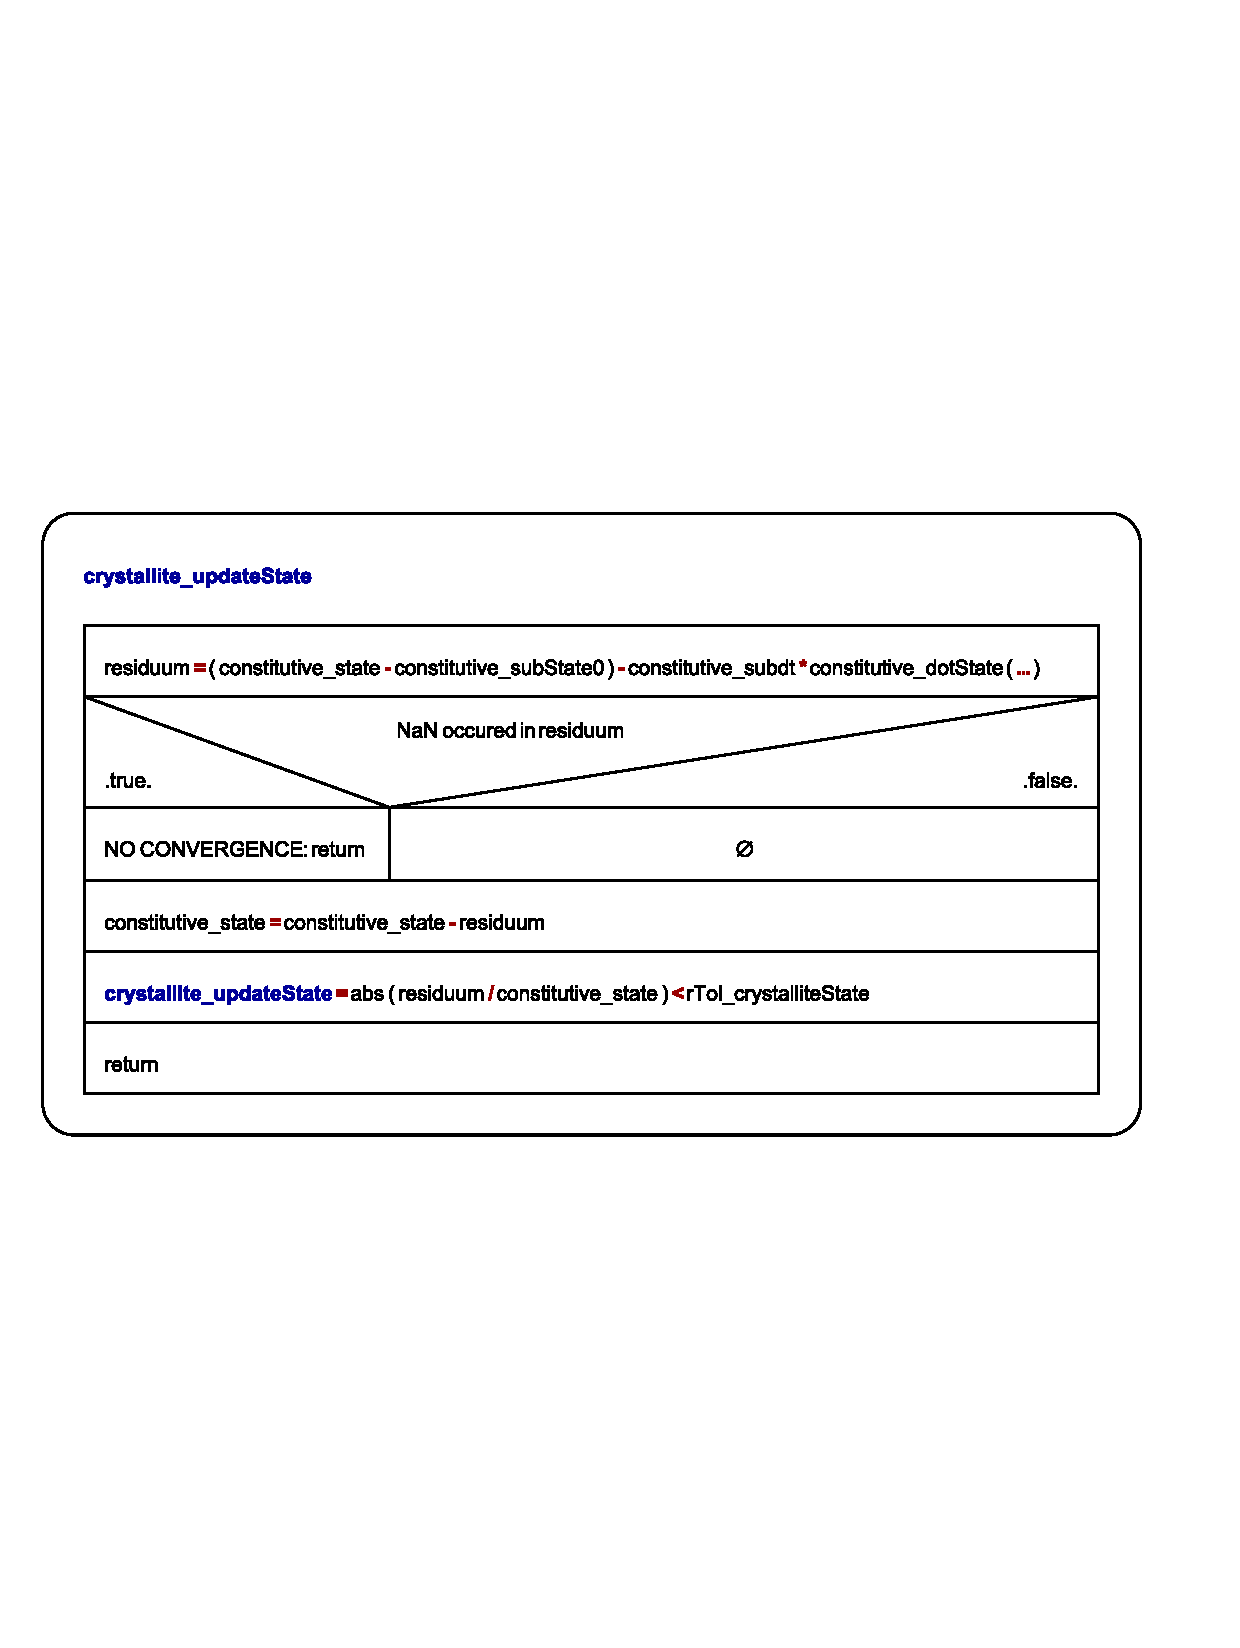
\includegraphics[width=0.80\textwidth]{crystallite_updateState}
\caption{updateState}
\label{fig:crystallite_updateState}
\end{figure}


% #################
\chapter{Homogenization schemes}
% #################

%\section{Introduction}
If more than one grain is simulated per integration point, a homogenization scheme is required to distribute the deformation gradient of the IP to the respective grains. The simplest choice is the \emph{isostrain approach} which simply consists in assuming the IP deformation gradient to be applicable directly to each grain. 
%\section{Isostrain homogenization -- Taylor's assumption}
%\section{RGC}

cite RGC papers...


% #################
\chapter{Constitutive Laws}
% #################

\section{phenoPowerlaw}
\subsection{The material file for phenoPowerlaw}
\section{dislotwin}
\section{The non-local model}

\section{The material file: material.config}


% #################
\chapter{Application notes for different finite elements systems}
% #################

\section{MSC.MARC/Mentat}
In MARC the CPFEM routine is interfaced through the {\ttfamily hypela2} subroutine. The routine {\ttfamily makeMe.py} produces the interface files such as {\ttfamily mpie\_cpfem\_marc2008r1.f90} that will can be called by the different MARC releases. 

Necessary changes in the submit scripts

Model definition for using the subroutine: In MARC, state variable 1 defines the temperature in Kelvin. State variables 2 and 3 define the homogenization and microstructure, respectively.

Analysis options to invoke: Large Strain, Updated Lagrange. For most problems, using a constant dilatation formulation is important for robustness of the simulations. 
%The analysis options are most conveniently defined through a procedure file.

\subsection{Utility scripts}
\begin{itemize}
\item marcAddUserOutput.py [<No. of UserVars>] marcinput --- adds UserVariables to the marcinput file under the post section
\end{itemize}

\subsection{Practical hints}
A copy of the subroutine on the home directory on the SAN makes the routine accessible from all workstations under /san/arbitraryfoldername/code/*.f90 .
Under windows it is beneficial to keep an additional local copy of the routine to work with TortoiseSVN, since the change of folder icons seems to not work on the SAN. 


\section{Troubleshooting}
\subsection{Inside out element error}
An inside out element error can occur if the number of increment is chosen too small. This was observed for revision 539 using the pheno-powerlaw constitutive formulation on a particle in mesh problem. 

\section{Abaqus}
Differences to Marc.


% #################
\chapter{Postprocessing of the results}
% #################

mentat, py\_post, gri, ParaView, TSL-OIM


% #################
\chapter{Worked examples}
% #################

Refer to the corresponding publications ...





\appendix
\cleardoublepage \phantomsection % set the hyperref anchor at the right position

% ########################
\chapter{Crystallographic orientations}
% ########################

\section{Bunge Euler angles}
\label{bunges}
Euler angles $(\varphi_1, \phi, \varphi_2)$---following the Bunge convention---rotate the sample coordinate system ($X$, $Y$, $Z$  or RD, TD, ND) into the crystal coordinate system ($x_\text c$, $y_\text c$, $z_\text c$). 
Three successive rotations are carried out in the following way \citep[p.~4]{Bunge1982}:
\begin{enumerate}
	\item Rotate by $\varphi_1$ around Z, to bring X into the $x_\text c$--$y_\text c$-plane. The new intermediate axes are $X^\prime$,  $Y^\prime$ and $Z$ (unchanged).
	\item Now rotate by $\phi$ around  $X^\prime$, to make $Z$ parallel with $z_\text c$. The intermediate axes are  $X^\prime$,  $Y^{\prime\prime}$,  $Z^\prime$.
	\item A final rotation by $\varphi_2$ around  $Z^\prime \equiv z_\text c$ makes the rotated axes then identical to the crystal axes.
\end{enumerate}

The rotation matrix can be calculated as
\[% Gottstein pg 55
\tnsr{g}=\left(\begin{array}{ccc}
\cos{\varphi_1}\cos{\varphi_2}-\sin{\varphi_1}\sin{\varphi_2}\cos{\phi} & \sin{\varphi_1}\cos{\varphi_2}+\cos{\varphi_1}\sin{\varphi_2}\cos{\phi}& \sin{\varphi_2}\sin{\phi}\\
-\cos{\varphi_1}\sin{\varphi_2}-\sin{\varphi_1}\cos{\varphi_2}\cos{\phi} & -\sin{\varphi_1}\cos{\varphi_2}+\cos{\varphi_1}\cos{\varphi_2}\cos{\phi}& \cos{\varphi_2}\sin{\phi}\\
\sin{\varphi_1}\sin{\phi} & -\cos{\varphi_1}\sin{\phi}& \cos{\phi}
\end{array}\right)
\]



\chapter{Related works}
\section{Publications}

\section{PhD thesises}
KuoDiss MaDiss ZaafaraniDiss

\bibliographystyle{plainnat}
\bibliography{MPIE_CPFEM_manual}

\end{document} 